\section{Background}
\label{sec:background}
In this section, we have discussed the traditional operations carried out in validating the accountability for a DNN model.
\paragraph{Forward Propagation.}  In this stage, a DNN model learns the features from the input. This stage includes random initialization, activation functions, feedforward, and loss function. A deep neural network can be represented as a fully connected graph as depicted in Figure \ref{fig:rq5}. This graph consists of nodes and edges. There is a value associated with the nodes and edge; these values are initially randomly initialized to start the training process. This step is very important as a wrong initialization parameter can hamper the learning process and take a longer iteration to reach optimality. Also, it is never a good idea to initialize them with zero as in the consecutive steps, the gradient will be computed as zero, and this will end up not learning anything from the input. The activation function has an impact on the computation; however, it does not change the probability distribution of the computation. The main purpose of the activation function is to convert the representation of the value corresponds to the nodes according to the need. Whereas the loss function computes the difference between the expected and the actual result.
\paragraph{Backward Propagation.} This is similar to the forward propagation, but only the difference is the way of computation. In this stage, the network operations are computed backward, and the derivative of each term has been computed to find the gradient that helps the learning process to localize the error and fix in the direction of the gradient.
%\paragraph{Seed.} A seed is a random number used when training DNN. The seed for DNNs tells them where to start in the sequence. Thus, Changing the seed means that changing the starting point of a DNN, which can lead to different outputs.
%\paragraph{Bias.} It is used to make sure if even when all the input is none, there will be activation in the neuron. Therefore, the value of bias is always 1. Moreover, it is an extra input to neurons, and it has its own connection weight. 
%\paragraph{Weights.} A weight represent the strength of the connection between units. For example, neuron A has greater influence over neuron B if the weight from node A to node B has a greater magnitude. The input will not change the output if the weights near zero. Moreover, negative weights mean increasing this input will decrease the output. Overall, a weight decides how much influence the input will have on the output.
\begin{wrapfigure}{R}{0.65\linewidth}
	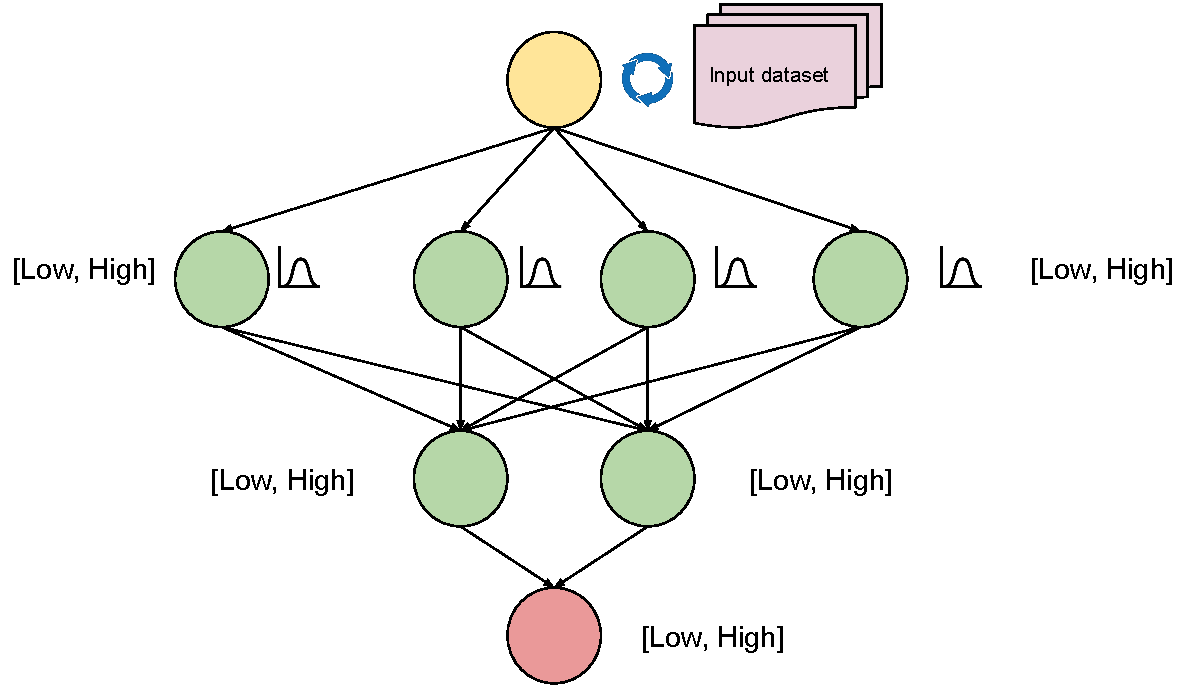
\includegraphics[width=\linewidth]{overview}
	\caption{Overview of a simple fully connected DNN model}
	\label{fig:rq5}
	%\vspace{15pt}
\end{wrapfigure}
